% -*- latex -*-
%%%%%%%%%%%%%%%%%%%%%%%%%%%%%%%%%%%%%%%%%%%%%%%%%%%%%%%%%%%%%%%%
%%%%
%%%% This TeX file is part of the tutorial
%%%% `Introduction to the PETSc library'
%%%% Victor Eijkhout, eijkhout@tacc.utexas.edu
%%%% copyright Victor Eijkhout 2012-2020
%%%%
%%%%%%%%%%%%%%%%%%%%%%%%%%%%%%%%%%%%%%%%%%%%%%%%%%%%%%%%%%%%%%%%

\sectionframe{Grid manipulation}

\begin{longversion}
\frame[containsverbatim]{\frametitle{Regular grid: DMDA}
DMDAs are for storing vector field, not matrix.

Support for different stencil types:

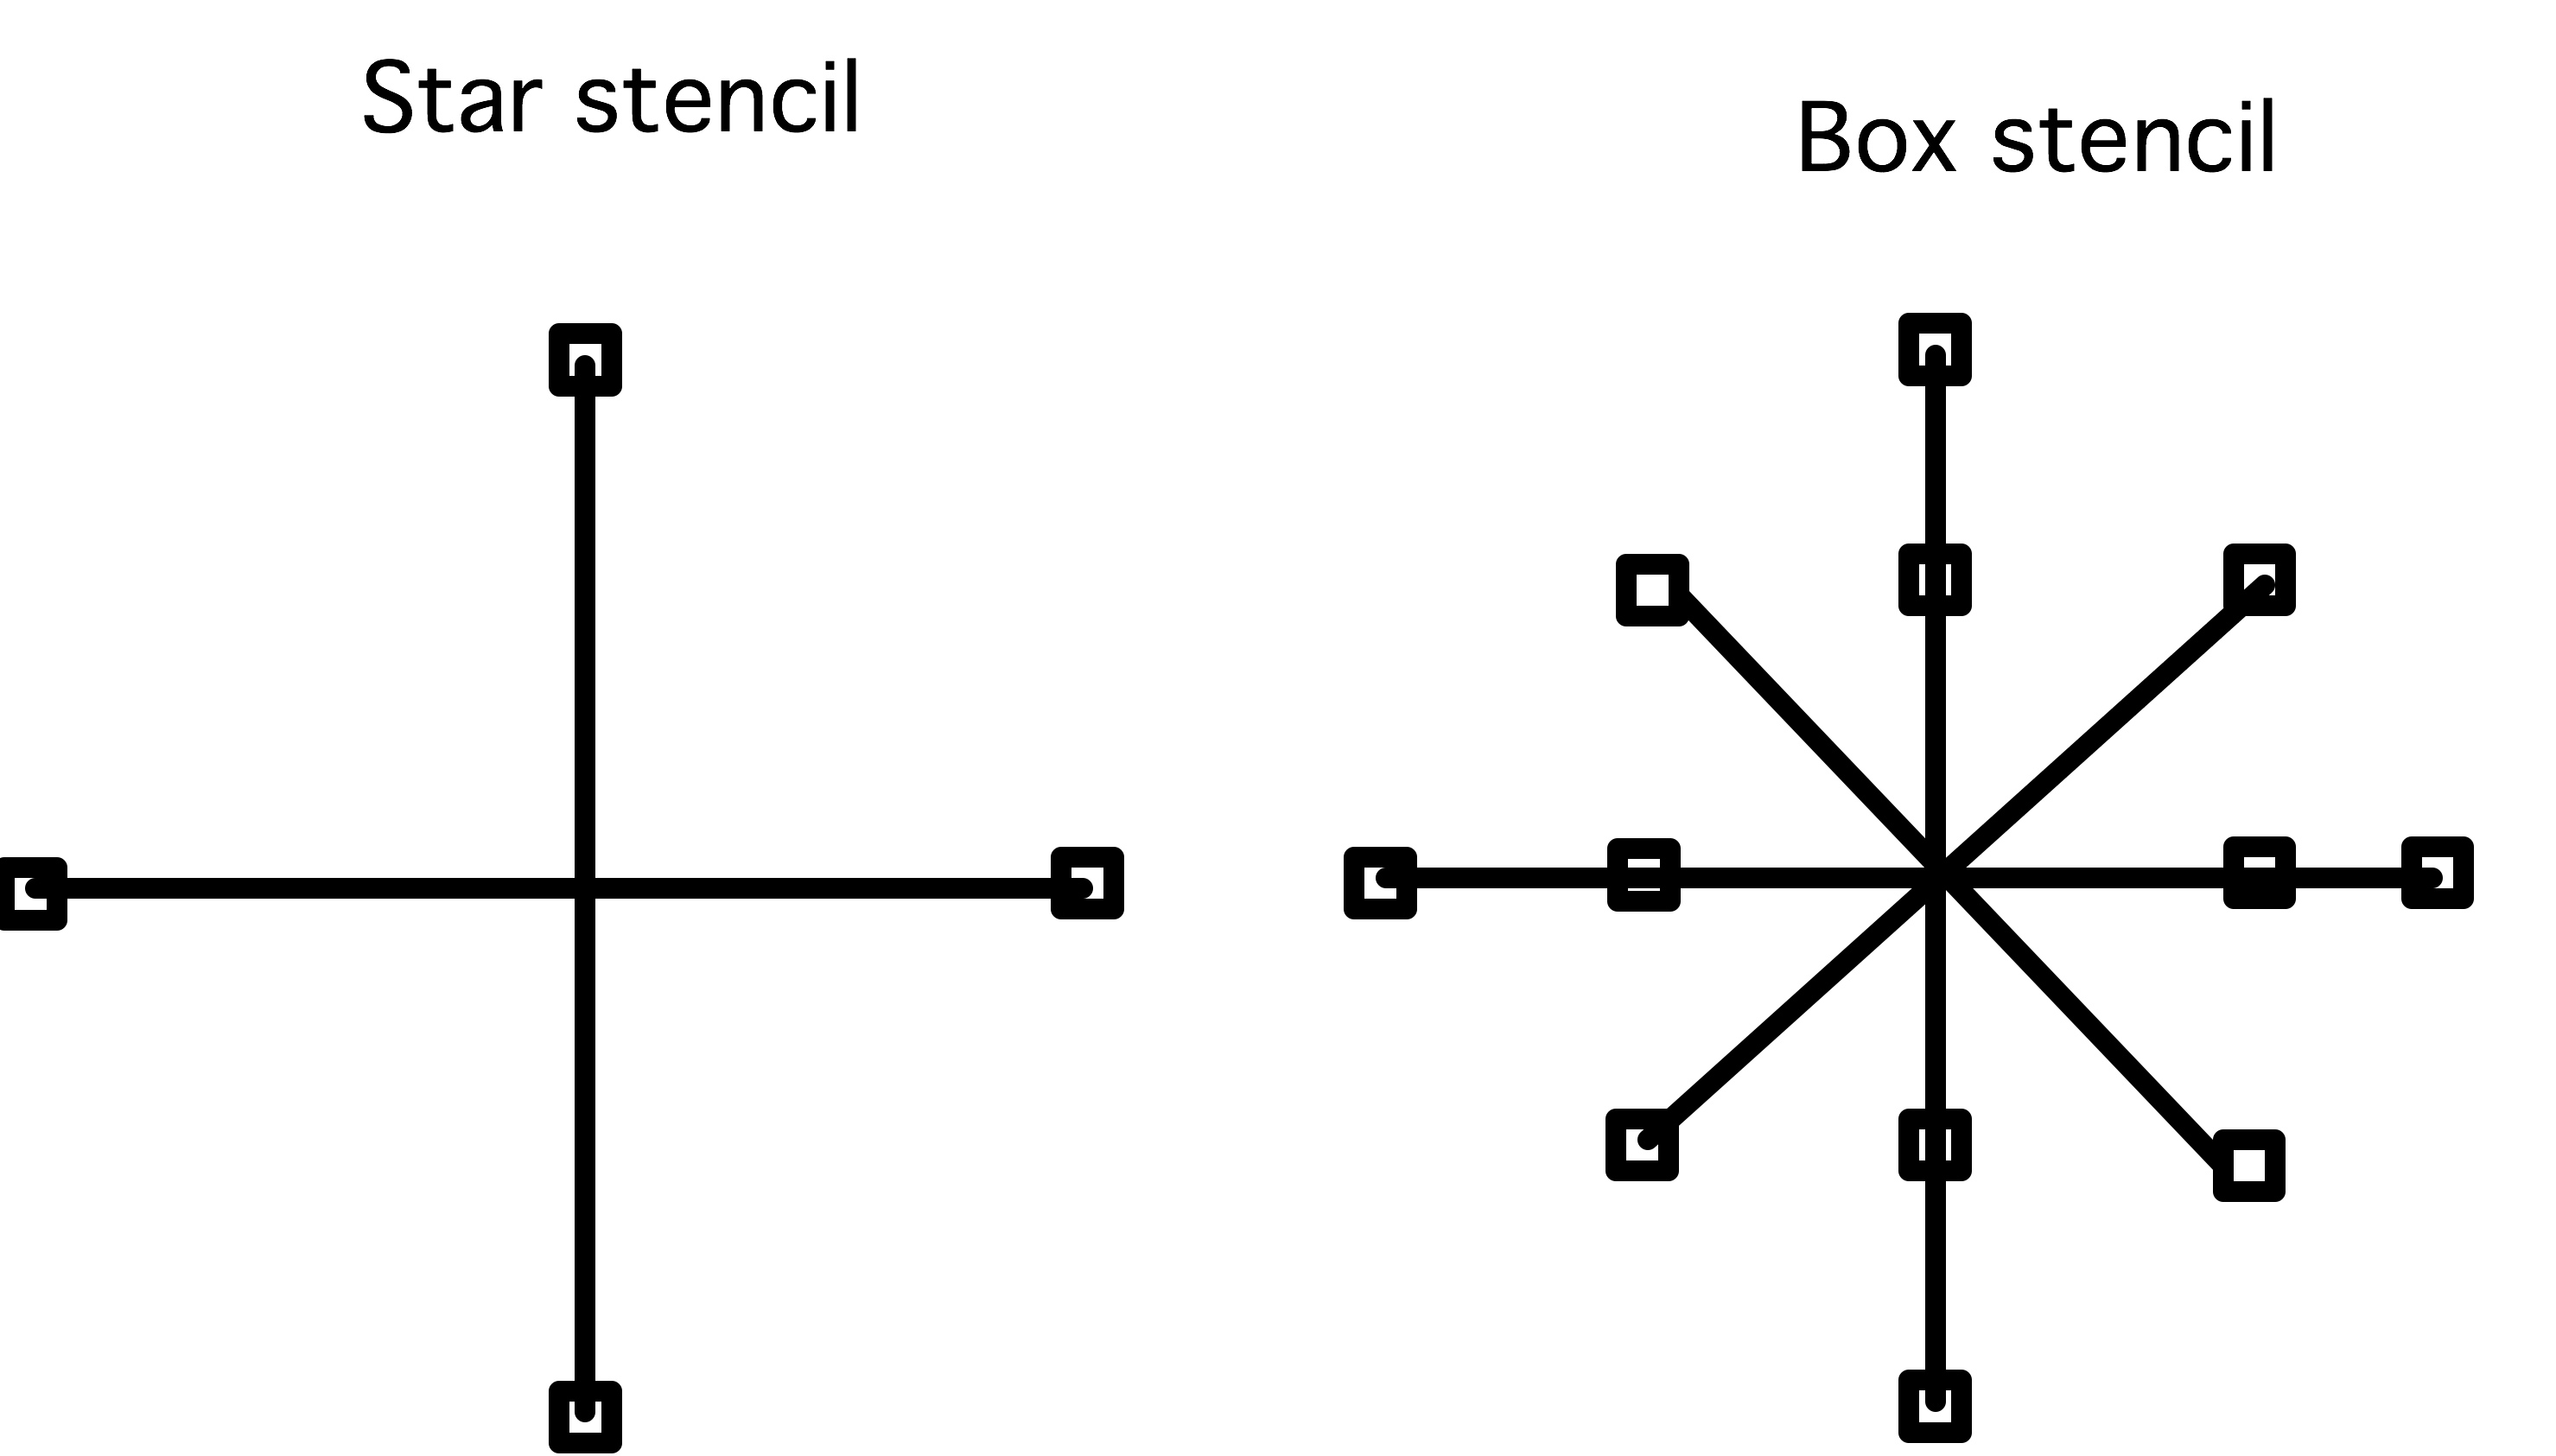
\includegraphics[scale=.07]{starbox}
}

\frame[containsverbatim]{\frametitle{Ghost regions around processors}
A DMDA defines a global vector, which contains the elements of the grid,
and a local vector for each processor which
has space for "ghost points".

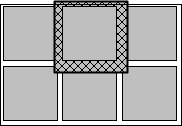
\includegraphics[scale=.6]{ghost}
}

\frame[containsverbatim]{\frametitle{DMDA construction}
\begin{lstlisting}
DMDACreate2d(comm, bndx,bndy, type, M, N, m, n, 
  dof, s, lm[], ln[], DMDA *da)
\end{lstlisting}
\footnotesize
\n{bndx,bndy} boundary behaviour: none/ghost/periodic

type: Specifies stencil\\
\n{DMDA_STENCIL_BOX} or \n{DMDA_STENCIL_STAR}

M/N: Number of grid points in x/y-direction\\
m/n: Number of processes in x/y-direction\\
dof: Degrees of freedom per node\\
s: The stencil width (for instance, 1 for 2D five-point stencil)\\
lm/n: array of local sizes (optional; 
Use \n{PETSC_NULL} for the default)
}

\frame[containsverbatim]{\frametitle{Associated vectors}
\begin{lstlisting}
DMCreateGlobalVector(DM grid,Vec *g);
DMCreateLocalVector(DM grid,Vec *l);

global -> local
DMGlobalToLocalBegin/End
    (DMDA da,Vec g,InsertMode iora,Vec l);

local -> global
DMLocalToGlobalBegin/End
    (DMDA da,Vec l,InsertMode mode,Vec g);

local -> global -> local :
DMLocalToLocalBegin/End
    (DMDA da,Vec l1,InsertMode iora,Vec l2);
\end{lstlisting}
}


\frame[containsverbatim]{\frametitle{Associated matrix}
Matrix that has knowledge of the grid:
\begin{lstlisting}
DMSetUp(DM grid);
DMCreateMatrix(DM grid,Mat *J)
\end{lstlisting}
Set matrix values based on stencil:
\begin{lstlisting}
MatSetValuesStencil(Mat mat,
  PetscInt m,const MatStencil idxm[],
  PetscInt n,const MatStencil idxn[],
  const PetscScalar v[],InsertMode addv)
\end{lstlisting}
(ordering of row/col variables too complicated for \n{MatSetValues})
}

%% \begin{frame}[containsverbatim]{Looping over the grid}
%% Loop over local part of the grid:
%% \begin{lstlisting}
%% DMDAGetCorners(DMDA da,
%%   PetscInt *x,PetscInt *y,PetscInt *z,
%%   PetscInt *m,PetscInt *n,PetscInt *p)
%% \end{lstlisting}
%% \end{frame}

\begin{frame}[containsverbatim]{Grid info}
\begin{lstlisting}
typedef struct {
  PetscInt         dim,dof,sw;
  PetscInt         mx,my,mz;    /* grid points in x,y,z */
  PetscInt         xs,ys,zs;    /* starting point, excluding ghosts */
  PetscInt         xm,ym,zm;    /* grid points, excluding ghosts */
  PetscInt         gxs,gys,gzs; /* starting point, including ghosts */
  PetscInt         gxm,gym,gzm; /* grid points, including ghosts */
  DMBoundaryType   bx,by,bz;    /* type of ghost nodes */
  DMDAStencilType  st;
  DM               da;
} DMDALocalInfo;
\end{lstlisting}
\end{frame}

\begin{frame}[containsverbatim]{Set values by stencil}
\begin{lstlisting}
DMDALocalInfo  info;
ierr = DMDAGetLocalInfo(grid,&info);CHKERRQ(ierr);
for (int j=info.ys; j<info.ys+info.ym; j++) {
  for (int i=info.xs; i<info.xs+info.xm; i++) {
    MatStencil  row = {0}, col[5 ] = {{0}};
    PetscScalar v[ 5 ];
    PetscInt    ncols = 0;
    row.j        = j; row.i = i;
    // diagonal element:
    col[ncols].j = j; col[ncols].i = i; v[ncols++] = 4.;
    /* boundaries: top row */
    if (i>0)         {col[ncols].j = j;   col[ncols].i = i-1; v[ncols++] = -1.;}
    /* boundary left and right */
    if (j>0)         {col[ncols].j = j-1; col[ncols].i = i;   v[ncols++] = -1.;}
    if (j<info.my-1) {col[ncols].j = j+1; col[ncols].i = i;   v[ncols++] = -1.;}
[et cetera]    
\end{lstlisting}
\end{frame}

\begin{frame}{DMPlex}
  Support for unstructured grids and node/edge/cell relations.

  This is complicated and under-documented.
\end{frame}

\endinput

% \frame[containsverbatim]{\frametitle{Indexing, setting, getting values}
% \begin{lstlisting}
% PetscScalar **f,**u;
% ...
% DMDAVecGetArray(DMDA da,Vec local,(void*)u);
% DMDAVecGetArray(DMDA da,Vec global,(void*)f);
% ...
% f[i][j] = u[i][j] - ...
% ...
% DMDAVecRestoreArray(DMDA da,Vec local,(void*)u);
% DMDAVecRestoreArray(DMDA da,Vec global,(void*)f);

% Global indexing, but only local entries are defined.

% DMDAGetCorners(DMDA da,int *x,int *y,int *z,int *m,int *n,int *p);
% DMDAGetGhostCorners(DMDA da,int *x,int *y,int *z,int *m,int *n,int *p);
% \end{lstlisting}

% (also global?)

% }
\end{longversion}

